\documentclass[a4paper,12pt,table]{article}
\usepackage[margin=1in]{geometry}
\usepackage{amsmath}
\usepackage{amssymb}
\usepackage{fancyhdr}
\usepackage[table,xcdraw]{xcolor}
\usepackage{float}
\usepackage{blindtext}
\usepackage{microtype}
\usepackage[hidelinks]{hyperref}
\usepackage{graphicx}
\usepackage[ruled,vlined]{algorithm2e}
\usepackage{color,soul}


\renewcommand{\arraystretch}{2.5}

\setlength{\parindent}{0cm}
\setlength{\parskip}{1em}
\pagestyle{fancy}
\fancyhf{}
\renewcommand{\headrulewidth}{0pt}
\renewcommand{\footrulewidth}{0pt}
\rhead{
}
\fancyfoot[R]{\thepage}
\graphicspath{ {C:/Users/sarya/Desktop/Semester 4/ISM/Report} }
\begin{document}

\begin{titlepage}
   \begin{center}
       \vspace*{6cm}

       \textbf{{\Huge Independent Study Module Report}}

	\vspace{5cm}

 {\Large An Investigation of Reinforcement Learning Algorithms for Mastering the Game of Santorini}

       \vspace{0.5cm}

       \vspace{1.5cm}


       \vfill



       \textbf{Aryan Sarswat -  A0200521E \\
		Lim Wei Liang - A0205466E \\
		Roy Chua Dian Lun - A0199930N \\ }

       \vspace{0.8cm}

      University Scholars Programme\\
       National University of Singapore\\

   \end{center}
\end{titlepage}


\tableofcontents
\newpage


\section{Introduction}

\subsection{Outline}

The advent of Artificial Intelligence has allowed mankind to transcend what we thought is humanly possible, and many different approaches have been developed to create machines which can perform intelligent tasks previously thought to be limited only to humans, such as driving a car. Furthermore these machines can do so at a speed and accuracy that transcend what the best humans can achieve. \par

One such method, known as Reinforcement Learning has seen increasing popularity recently, with one of its most recent successes being its use by Google DeepMind to develop AlphaGo, a computer programme which has defeated the Legendary Go player Mr Lee Sedol, the winner of 18 world titles. In essence, the technique of Reinforcement Learning works by training “agents" to take “actions" in an environment that maximise a predetermined “reward".

\subsection{Objective}

The objective of this ISM is to develop an agent which can effectively play the board game Santorini. This is largely novel as there is no accepted standard in developing an agent in the game of Santorini. \par

A wide variety of reinforcement learning techniques that have been shown to be effective in playing other two-player zero-sum games have been implemented, tested and compared with one another. Firstly, more traditional approaches making use of linear, feature-based, value function approximation combined with reinforcement learning and minimax search were implemented and tested. Then, more cutting-edge methods such as non-linear value function approximation were investigated using Artificial Neural Networks (ANNs) and Convolutional Neural Networks (CNNs), as well as a form of simulation-based search and self-play reinforcement learning shown to be successful in highly complex domains - Monte Carlo Tree Search. Finally, we attempted to combine parts of each approach in order to cope with some of the limitations encountered. \par

Evaluation of the implemented models was undertaken by pitting them against each other, while also taking into account the time taken for each move. Finally, we will consider some of the limitations of our investigation into reinforcement learning techniques for playing Santorini.

\section{Santorini}

\subsection{Game Rules}

Santorini is a 2-player board game on a 5x5 grid, with 3 distinct pieces: building blocks, the worker and a dome. Each turn, a player will move his worker to an adjacent tile, then place a building block on a tile adjacent to the moved worker. The building blocks can be stacked up to 3 levels. The worker can only traverse to an adjacent tile that is within 1 level of the worker’s current tile or if it is jumping down levels (i.e. if the worker is on level 1, he can only move to an adjacent tile of level 0, 1 or 2). When there are 3 building blocks on a tile, a dome can be placed on top of the blocks to prevent another player from reaching level 3. The worker has to traverse from the ground level (level 0) to level 3 in order to win the game. Another way to win is to force the opposing worker to have no adjacent tiles to move to. \par

\subsection{Game Code}

An Object-Oriented Programming (OOP) approach was employed to simulate the board-game, as it was deemed as the most “user-friendly” approach, allowing ease of code review and overall game design. The main objects that were instantiated were: 1) Worker, 2) Square, 3) Board, and 4) Player. All of the game’s code was done in Python 3.9. \par

\begin{enumerate}
    
    \item \textbf{Worker Class}
    \newline
    The Worker class is a base class, representing a Worker object on the Board. The worker has two pieces of information stored: the player it belongs to, and its position on the board (represented by a tuple of x-y coordinates). It allows us to immedientely determine the location of the workers to calculate possible future moves.
    
    \item \textbf{Square Class}
    \newline
    The Square class represents a “square” on the board, having immutable x-y coordinates (represented as a tuple) as an attribute. It possesses two pieces of information: the level of buildings (represented as an integer ranging from 0 to 4), and whether a worker is present (represented by either a Worker object or None).
    
    \item \textbf{Board Class}
    \newline
    The Board class represents the entire state of the board game, which is the main object used for interaction with the players. The space of the board (a 5x5 grid) is represented as a list of 25 Square objects. The Board class has methods for checking terminal states and validity of player actions.
    
    \item \textbf{Player Class}
    \newline
    The Player class is a super class for all agents and human players. It possesses information about its Worker locations, as well as two methods: one to place its 2 workers at the start of the game, and one to simulate an action (movement of a worker piece, followed by placement of building). \par

\end{enumerate}
A simulation of the board game will start with the creation of a Board object and 2 Player objects (either human or AI), and initialize worker placement depending on the Player object. The players (starting from Player A) will take turns doing an action until a terminal state is reached, where either player wins, of which the script will terminate for a single simulation. \par

\section{Methods employed to create AI Agent}

\subsection{Traditional Approaches using Minimax Search coupled with Linear Value Function Approximators and Reinforcement Learning}

\textbf{Minimax Search}
\newline
Minimax Search is a well-established idea that can be used to create a game-playing AI. In Minimax Search, one player is assigned to be the maximizing player, while the other is the minimizing player. \par

In the ideal case, each time it must make a decision the agent will construct a search tree starting with the current game state as the root node, branching into all possible states that the game can progress to depending on the moves that the agent and opponent make. The tree reaches a terminal node when either player wins. These winning nodes are assigned either an arbitrarily large positive or negative value depending on which player has won (in our case, we used 9999 for the maximizing player and -9999 for the minimizing player). \par

Then, starting from the 2nd last row of the search tree, the best possible move for each player at a branching node is determined by them selecting the move that would lead to either the maximum or minimum possible value amongst the child nodes, depending on which player they are. This represents each player playing perfectly and allows us to assign values to non-terminal nodes. Going up the search tree, we eventually reach the root node where we can now determine the best possible move to make. Such a state of play is optimal and achieves the Nash equilibrium. \par

Unfortunately, in most games (Santorini included), it is not possible to construct a search tree up to the winning nodes, given how the large number of possible moves at each state contribute to large branching factors in the search tree. Santorini specifically has a branching factor of about 30-100, and it is larger at the start of games when more moves are possible. Taking the average to be around 50 possible moves at each state, a Minimax Search tree would have an exponential time complexity of $O(50^n)$, where $n$ is the search depth. Hence, it is only possible to search up to a fixed depth, and a means of approximating the state value is required at the terminal leaf nodes which do not represent a win. \par

\vspace{1.5cm}
\textbf{Linear Value Function Approximation}
\newline

One simple and effective way of approximating the value of a given game state would be using a linear value function approximator. Linear approximators have a preset list of features used to evaluate a game state, as well as an array of weights, which represent the value of each feature. The state value will then be calculated by taking the dot product of the feature vector and weights vector \hl{(insert eqn?)} Such linear approximators have seen great success in other traditional board games, most notably in Chess, where IBM’s Deep Blue beat the reigning world champion Garry Kasparov. \par

As a preliminary investigation, a simple linear value function approximator for Santorini was constructed, comprising of the following 8 features that were normalized from 0 to 1:
\begin{enumerate}
    \item Number of workers on Level 0
    \item Number of workers on Level 1
    \item Number of workers on Level 2
    \item Centrality - Average worker distance from the board centre
    \item Repeat features 1 - 4 for the other player
\end{enumerate}

These simple features were constructed using some pre-existing knowledge and experience of the gameplay, being highly representative of the strength of a player’s position. Worker height was considered since after all the game is won by having workers gradually ascend to level 3, and centrality because a player tends to have more possible moves and opportunities when their workers are at the centre of the board rather than at the edges. Pre-existing knowledge was also used to come up with a set of weights for each feature that seem to make logical sense, which were [0,2,4,-1,0,-2,-4,1]. This essentially means that greater heights are prioritized more (i.e. getting to Level 2 $>$ Level 1 $>$ Level 0), as well as keeping workers closer to the centre. Playing against an AI using these weights, we observe that it behaves extremely logically, and is fairly competent especially with deeper search depths. However, our initial implementation was greatly hampered by our inability to perform deep searches at acceptable speeds - a search at depth 3 took nearly 60 seconds just to come up with a move. \par

\textbf{Optimizations in Minimax Search}
\newline
It was also observed that one major factor greatly contributing to the strength of a game playing AI would be the search depth that it undertakes. Testing using the same set of weights, an AI with a minimax search depth 3 won 95\% of games against an AI of minimax search depth 2. Hence, it would be highly beneficial to first make optimizations in this area before attempting to train an AI using reinforcement learning. \par

The first optimization technique implemented was alpha-beta pruning, which is a method of reducing the time complexity of a full minimax search by skipping calculations of nodes and entire branches in the search tree which are certain not to affect the final outcome. Additionally, further optimizations can be made to enhance alpha-beta pruning itself - one of these is known as move ordering, which involves sorting the list of all possible moves generated based on a heuristic so that moves likely to be stronger are considered first. This would result in pruning taking place earlier in the search tree, and hence fewer calculations being made. For Santorini, the list of all possible moves generated was sorted based on the sum of squares of the current player’s worker heights, as typically moves that bring the worker up to higher floors tend to be stronger. Squaring the height automatically prioritizes moves to level 3 over level 2, 1 and 0. \par

Furthermore, the game’s implementation was partially rewritten based on observed bottlenecks in the original code, one of which was due to the use of the rather slow deepcopy function when generating all possible moves. This problem was compounded as a minimax search tree easily generates and searches through a large number ($>10000$) possible moves every time the agent has to make a decision, and as mentioned above this number increases exponentially with search depth. Instead, the game state was changed to be represented by numpy arrays and lists of tuples while searching through the large number of possible moves, as they could be copied much more efficiently. \par

Collectively, these optimizations allowed for an optimized minimax search tree of depth 4 to be generated in about 2 seconds, as compared to the same amount of time needed just for depth 2 previously. \par

\textbf{Learning Feature Weights thorugh Reinforcement Learning}
\newline

After the linear value function approximator was created and the search algorithm optimized, the possibility of the agent learning the weights through existing reinforcement learning techniques was investigated. In the paper ‘Bootstrapping from Game Tree Search’, Veness et al., introduced new and improved algorithms for performing minimax search bootstrapping, which is the idea that a value function approximator can approximate the minimax value resulting from a deep game tree search without actually using computational power to perform said search. Game playing performance would then be significantly improved due to the greater effective search depth resulting from both the search actually performed and the bootstrapped search from the approximator. The algorithms introduced, applied to a linear value function approximator of 1812 features, were demonstrated to be capable of learning from self-play and with randomly initialized weights in Chess, achieving master-level performance. \cite{Bootstrapping from Game Tree Search} This approach combines both reinforcement learning as well as the idea of searching for good moves using minimax, which is important in ‘highly tactical domains’ \cite{Bootstrapping from Game Tree Search}. Hence, we apply the same approaches for the purpose of playing Santorini, which is also a tactical 2-player game. \par

The two main algorithms introduced in the paper, named RootStrap and TreeStrap, were thus implemented and used to train the weights for our linear function approximator. Each of these algorithms were used in 100 training games of self-play, starting from randomly initialized weights. A minimax search tree of depth 3 was used, (we take depth to increase by 1 when either player makes a move) as well as the same learning rates used in the research paper ($10^{-5}$ for RootStrap and $10^{-6}$ for TreeStrap) The sketch of these training algorithms are given below, based on how they were described by Veness et al. \par

Both algorithms update the linear value function approximator’s weights using ‘stochastic gradient descent on the squared error’ between the approximator’s predicted value, and the actual minimax search value. While RootStrap updates only the root node towards the calculated minimax value at that node, TreeStrap updates all nodes within the search tree towards their respective minimax search values. \par

\bigskip
Let the state value given by the linear approximator be given by V\_approx.(State, Weights)

\medskip

\begin{algorithm}[H]
    \SetAlgoLined
    \KwResult{Weights Trainied}
    Randomly initialize starting weight vector W from -1 to 1 for each element\;
    \ForEach(){Game}{
        \ForEach{state S}{
            Construct a minimax search tree of specified depth, evaluating terminal nodes using V\_approx(child\_state, W) \;
            Find value V given by the minimax tree of the current state S \;
            $Error \leftarrow V - V\_approx(S,W)$ \;
            $W \leftarrow W + learning\_rate \times error \times feature_vector of state S$ \;
            Pick best move by taking the argmax of minimax values of child nodes \;
            Execute move \;
            \eIf{either player wins}{
                Break out of inner loop\;
            }{
                Carry on with next state as the other player \;  
            }
        }        
    }
    \caption{Algorithm for RootStrap}
\end{algorithm}

\begin{algorithm}[H]
    \SetAlgoLined
    \KwResult{Weights Trainied}
    Randomly initialize starting weight vector W from -1 to 1 for each element\;
    \ForEach(){Game}{
        \ForEach{state S}{
            Construct a minimax search tree of specified depth, evaluating terminal nodes using V\_approx(child\_state, W) \;
            $Total_update \leftarrow 0$ \;
            \ForEach{State $S'$ in the tree}{
                Find value $V’$ given by the minimax search tree of that state $S’$ \;
                $Error \leftarrow V’ - V\_approx(S’, W)$ \;
                $ total\_update \leftarrow total\_update + learning\_rate \times error \times feature\_vector$ of S \;
            }
            $W \leftarrow W + total\_update $\;
            Pick best move by taking the argmax of minimax values of child nodes \;
            Execute move \;
            \eIf{either player wins}{
                Break out of inner loop\;
            }{
                Carry on with next state as the other player \;  
            }
        }        
    }
    \caption{Algorithm for TreeStrap}
\end{algorithm}

Having implemented and tested the algorithms, it was found that they were fairly effective in learning a set of weights despite being trained only by self-play and starting from random initial weights. After 100 games, the performance of both TreeStrap and Rootstrap’s trained weights was fairly close to that of the manually tuned weights, showing evidence that these algorithms were indeed able to learn from automatically generated experience. \par

That said, since the linear function approximator trained through Reinforcement Learning does not yet manage to surpass the one tuned manually, it is clear that further optimizations will have to be made to improve the strength of the linear approximator and learning algorithms. \par

\textbf{Further Improvements to the Linear Approximator-Based AI}

As the basic minimax search, as well as reinforcement learning techniques used are effective despite the very limited linear value approximator, it would then be prudent to extend the number of linear approximation features to allow for a more informative state value approximation. (Currently In-Progress) \par

Additionally, there are also additional optimizations that may be made to further increase the speed of the minimax search, such as transposition tables for repeated moves, and a heuristic for enhancing alpha-beta pruning known as the killer heuristic. The variant of TreeStrap used in our testing also only used the regular minimax search tree without alpha-beta pruning, which is slower to train, as the variant described in the research paper which used alpha-beta pruning required an implementation of transposition tables which we had not implemented. \par


Finally, to create an AI that truly learns on its own without requiring prior experience for feature creation, the possibility of an algorithm that generates and evaluates its own linear features based on commonly encountered patterns in the game state could be explored, although such a problem may be more easily solved through non-linear value function approximation methods, such as ANNs and CNNs. \par


\subsection{Neural Networks (Value Function Approximation)}

Using Linear Value Function Approximation with minimax is an extremely effective process. In games where the branching factor is not very large, minimax can lead to optimal gameplay by the AI agent. However, due to the relatively large branching factor of Santorini (128 moves per turn), a reasonably fast AI agent can play by looking up to 4 states maximally. This severely handicaps the performance of the AI. This is one of the main reasons to attempt to use a Neural Network to predict the value of a state instead. \par

Neural Networks are essentially seen as universal function approximators, which can be used to mimic any function. Thus by using the minimax algorithm we can find the true value of a state and use that as our training data. This training data will be fed into the neural network which will adjust its weights and bias to be able to create a function which can accurately determine how strong a certain state is. This will increase the speed at which our agent can predict the value of a state and consequentely the optimal move. Since the minimax algorithm determines the value of the state by back propagating the value from a terminal state, there is no need to look ahead further states as they are already accounted for. This aspect of Neural Networks as function approximators significantly speed up the “thinking-time” of our agent. \par

One Hot Encoding was employed to turn the board state into a flattened array of size $[1,325]$ containing only ones and zeros. This was used to ensure that the height of the building is not given priority due to its large numbers (1-4). \par

\paragraph{ANN Architecture}
\begin{enumerate}
    \item \textbf{Input}
    \newline
    Consists of a 1,325 layer of Neurons as each board state contains 25 squares and there are 13 unique states thus a hot encoded flattened matrix would have 325 ones and zeros.
    \item \textbf{Neuron Layers}
    \newline
    This is actually a hyperparameter which we can change, for our experiments there was one hidden layer consisting of 256 input neurons and 64 output neurons. This layer was chosen arbitrarily.
    \item \textbf{Output}
    \newline
    The output consists of a tensor with one value. This value is between $[-1,1]$ inclusively. The higher its value is the better the state is for Player 1 and the lower it is the better the state is for Player 2. A value of 0 implies that the state is equally strong for both players.
    \item \textbf{Activation Functions}
    \newline
    The Rectified Linear unit (ReLU) activation function was employed to linearize the function and reduce its computational complexity. The Tanh function was also used in the output layer to ensure that the output was between $[-1,1]$. This not only squashed the results into this range but also did it proportionally. Thus if the value of a state is extremely large it would be reduced to 1 which can be interpreted as a completely winning state for Player 1.
    \item \textbf{The Loss Function}
    \newline
    The Mean Squared Error loss was employed, this ensured that the state values did not explode as it heavily punishes large differences between the true value and the value predicted by the neural network.
    \item \textbf{Optimizer}
    \newline
    For updating the weights of the Neural Network the Stochastic gradient descent (SGD) was employed. Due to the large number of Neurons in each layer and the weights associated with each of these neurons, SGD is an appropriate optimizer as it reduces the computational burden allowing us to achieve faster training for a trade off of lower convergence rate.
\end{enumerate}

\begin{figure}[h!]
    \begin{center}
        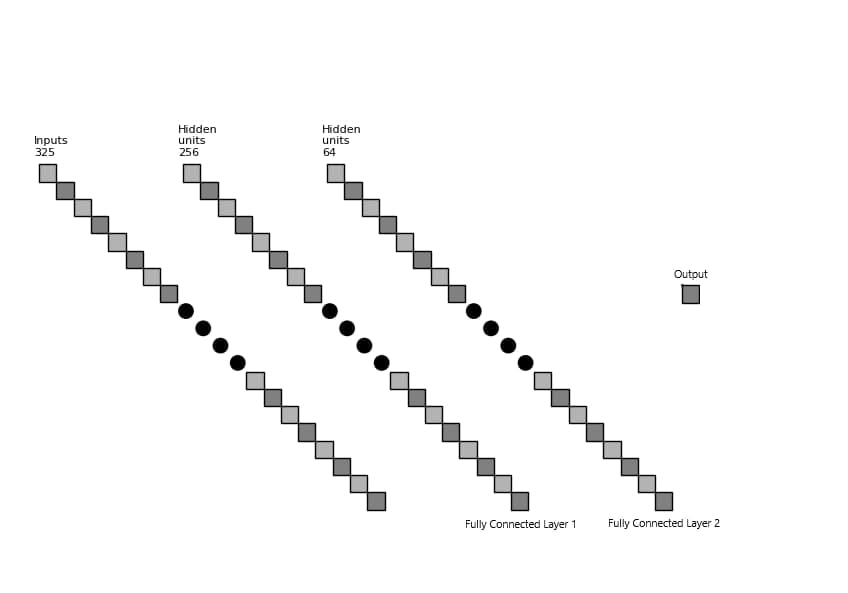
\includegraphics[scale=0.7]{ANN_Architecture.jpg}
        \caption{ANN Architecture}
        \label{fig:}
    \end{center}
\end{figure}


\subsection{Neural Networks with Convolutional Layers (Value Function Approximation)}

In order to make a value function approximator that is capable of converting board information to a state-value, a Convolutional Neural Network (CNN) was used to attempt to produce an accurate state-value given a board state. A CNN is capable of extracting relevant information from a multidimensional array.  It is a type of neural network that is commonly employed in fields of Computer Vision, such as feature detection of images. One common example is facial recognition technology, where a CNN is trained and employed to detect facial features.   \par

The rationale of employing a CNN in the determination of the state-value of a board, is mainly due to the capability of a CNN in retaining the 2-dimensional structure of an “image” of a board, whilst generating and preserving 2D spatial features that a normal ANN is not capable of. This is because a board is fundamentally 2-dimensional in nature, and the player is traversing in a 2D-board space (3D if the buildings are included). Therefore, features of the Santorini board, like the grouping of high-level buildings, or the proximity of a player to a building, is better extracted by a CNN rather than a simple 1D neural network structure. The feature extraction capability of a CNN is pivotal in determining how much “value” the board is to a player. \par

\textbf{CNN Architecture} 

The neural network was split into two distinct sections, the CNN layers (for feature extraction) and the ANN layers (for state-value determination).   \par

\begin{figure}[h!]
    \begin{center}
        \includegraphics[scale=0.4]{CNN_Archi.png}
        \caption{CNN architecture for first value function approximator}
        \label{fig:}
    \end{center}
\end{figure}

\begin{enumerate}
    
    \item \textbf{Input}
    \newline
    From the board, two sources of information were determined to be essential for the neural network to output an accurate state-value: worker position and building level. Hence, the input layer had 2 input features. The board was converted into 2 layers. Each layer is a 2-dimensional $5\times5$ array, representing the board structure. The first layer consisted of building data, where the possible building levels of 0 to 4 were min-max normalized (0 representing ground level, 0.25 representing level 1 etc). The second later consisted of worker data, where the player’s worker was denoted as 1, and the opponent’s worker was denoted as -1. 
    
    \item \textbf{Output}
    \newline
    The output was a tensor with a single value that represented the state-value of the board, with the maximum value of 1 being favourable for the player (aka a winning state) and the minimum value of -1 being not favourable.
    
    \item \textbf{CNN Layers}
    \newline
    The first CNN layer had an input feature value of 2, representing the building levels and worker positions. It outputted 16 feature channels, with a default stride value of 1. The second CNN layer had similar hyperparameters to the first layer, the only difference being the input features to be 16, corresponding to the out channels of the first layer.
    
    \item \textbf{Batch Normalization}
    \newline
    Batch normalization was implemented after every convolutional layer to coordinate the updating of weights at the end of every batch.
    
    \item \textbf{Pooling}
    \newline
    Pooling was not implemented in the CNN as the value function should retain as much information about the board as possible. 
    
    \item \textbf{Kernal Size}
    \newline
    A kernel size of 3 was adopted to capture the possible features of the board, as the worker could move in the adjacent 8 squares, hence the features that are extracted will be more relevant for the player’s worker.
    
    \item \textbf{Padding}
    \newline
    Padding with value of 1 was used to capture the information of the board corners more accurately.
    
    \item \textbf{Activation Function}
    \newline
    The Rectified Linear unit (ReLU) activation function was adopted for both the CNN and ANN layers (bar the second ANN layer), for less computational complexity and its linear behaviour.

    \item \textbf{Loss Function}
    \newline
    The Loss Function used was the MSE loss function, with the rationale similar to that of the ANN (as explained in Section \_\_).
\end{enumerate}

\textbf{Training of the first CNN Model}
\newline
The first CNN model was trained on a random agent (who made random worker movements and worker placements) for 5000 iterations. Each iteration represents a complete game of Santorini. For each state, the CNN agent will generate all possible next states, evaluate the states through the CNN, and output the state-value for each possible state. Based on an epsilon-greedy policy, it will then either make a random move, or make a move based on the state with the highest state-value. The state-value of the next state (either the random state or the state with the highest state-value) is saved in an array for backpropagation at the end of the iteration. As the reward given to the agent is only known at the end of the iteration, there is no update of weights to the CNN until the end of one iteration. \par

\begin{algorithm}[H]
    \SetAlgoLined
    \KwResult{Model Trainied}
    \ForEach(){Episode}{
        \While{game is not terminal}{
            Generate all possible states\;
            Generate all possible states-values for all states\;
            r $\leftarrow$ generate random number\;
            \eIf{r $>$ $\epsilon$}{
             Make action with the highest state-value\;
             }{
             Make random action\;
            }
            Store state-value of action made\;
            }
            $\epsilon$ $\leftarrow$ $\epsilon$ $\times$ ($\epsilon$ - decay)\;
            R $\leftarrow$ 1 (Agent Win) or -1 (Agent Loss)\;
            Backpropagate loss based on R\;          
    }
    \caption{Training CNN Model}
\end{algorithm}

\subsection{Monte Carlo Tree Search}
The Monte Carlo Tree Search algorithm is a variant of the standard Monte Carlo method where a search tree is constructed creating a sort of policy network for an agent to follow. It relies on rollouts to be able to successfully determine the value of a state. This is a very popular algorithm used in many board games; It was successfully implemented by researchers at Deep-Mind to develop AlphaGo an AI which was able to reach grandmaster level ELO at the game of GO. Monte Carlo Tree search is executed by 4 key steps; Selection, Expansion, Simulation and Backup. In one run of the algorithm, first Selection occurs and if the node is a leaf node (i.e has no children) it is expanded, after which a number of games are simulated from that leaf node, finally the values obtained from simulating these games are back propagated up to the root node. These four steps will be elaborated upon in detail below:

\begin{enumerate}
    \item \textbf{Selection:} \\
    Beginning at the root node, select a child node based on a heuristics which involve the visit count and value of the child state. For our experiment the Upper Confidence Bound (UCB1) was utilised. More specifically the UCB1 algorithm was used where along with the value of the state the number of visit of the child node and the parent node are also used to determine the criteria for selecting a child node. This algorithm allows for the selection of nodes which have not been visited and thus promotes exploration. This algorithm also contains a hyperparameter $c$ which is known as the exploration parameter and it is usually determined empirically, however we have used the accepted theoretical value of $\sqrt{2}$.
    \[v_i + c\sqrt{\frac{\ln{N_p}}{n_i}}  \]
    
    \item \textbf{Expansion} \\
    Once a leaf node is reached, the tree is expanded by adding children to the leaf node, these children are all the possible next states which may follow. This allows for the growth of the search tree. However if the leaf node is terminal it will not be expanded and in some cases one may choose not expand a leaf node completely.
    
    \item \textbf{Simulation} \\
    From the selected node or from a node which has been expanded, a complete episode starting from that node is simulated until the state is terminal. After which a reward is returned. This is also known as a rollout and the games are simulated with a certain policy; this policy could be a Linear Value Function, a random Policy or even a policy from a Neural Network which has been trained with expert games. Other than the node selected for the simulation, none of the other states in the simulation are stored, this significantly reduces the memory requirements compared to other methods such as Q-tables.
    
    \item \textbf{Backup} \\
    The return obtained from the simulated episode is the backed up the path taken to reach the leaf node or if it is the first node in the tree it used to initialize the value for the node. These values are then added up for each simulation in each node in a value sum variable, this will provide an indication how good or bad the state is. This is one of the key steps of the MCTS algorithm as instead of using randomly generated episodes, where the goal is to explore as many states as possible, it enriches this data and even though lesser states are explored, the data contains more refined information than that of a randomly generated episode.
\end{enumerate}

The figure below visually depicts how the algorithm runs \par

\begin{figure}[h!]
    \begin{center}
        \includegraphics[scale=0.65]{MCTS.png}
        \caption{One iteration of MCTS algorithm \cite{Reinforcement learning: An introduction}}
        \label{fig:}
    \end{center}
\end{figure}

\begin{algorithm}[H]
    \SetAlgoLined
    \KwIn{root}
    \KwOut{root}
    \KwResult{One Iteration of MCTS}
    \While{time/resource left}{
        \eIf{root is not expanded}{
            Expand Root\;
        }{
            $search\_path$ $\leftarrow [root]$\;
            $current\_node$ $\leftarrow$ root\;
            \While{$current\_node$ is expanded}{
                $current\_node$ $\leftarrow$ Select child from $current\_node$\;
                $search\_path$.append($current\_node$)\;
            }
            \For{Simulation $\in \{1,2,3,....., \text{Number of Simulations}\}$}{
                Reward $\leftarrow$ Rollout from $current\_node$\;
                Backpropagate Reward\;
            }
            \If{$Current\_node$ is not terminal}{
                Expand $current\_ node$\;
            }
        }
    }       
    \caption{Monte Carlo Tree Search}
\end{algorithm}

This algorithm continues to run until either a time limit is reached or some other computational resource such as memory is depleted. After the algorithm stops running the tree can be used as policy to be able to play games. For each node, the child node with the highest value can be selected, this works because if the visit count and the value of the state is high it implies during the simulation the tree had often selected this node, which means that it often wins in this state. \par

In addition to the above, the previous tree can be improved upon by selecting a leaf node which has not terminated and setting that node as the new root node to construct another MCTS tree. This will allow for greater exploration and better approximation of the value of states. However due to our computational constraints we were unable to run the MCTS algorithm for a significant upon of time, this is due to the fact that for the value of any node to converge we need a high number of simulation and this is not easily achievable on standard computers as they make take upto 4 to 5 days to complete the construction of one MCTS tree. Thus we developed a variation of the MCTS tree which considers the breadth of the tree instead of a depth. \par

The Algorithm is as follows: for each node, all the child nodes are selected one by one and for each of these node games are simulated to obtain a value of how good this state is, this value is normalized by the number of games simulated. After all the games have been simulated for all the child nodes, using the UCB1 algorithm a child node is selected which has the highest value, this child node then becomes the new root node. And for each iteration this repeatedly results in a higher depth explored. This algorithm significantly cuts down on the computational resources required, however this comes at a cost; since we are using the new child nodes as the new root nodes for another tree, we are essentially doing a one step look ahead, the values are not backed up all the way to the root node, this reduces the chances of the value of the state to converge. Furthermore it constricts the number of nodes which explores as it only searches down the path with the highest UCB1 value. \par


\subsection{Combining the Above}

In an attempt to address the limitation of each of the methods described above and the lack of experiment games we decided to combine the defining aspects of each method into one model. This was done using the MCTS tree to generate a game tree using the Linear Reinforcement agent’s policy for the rollouts. Multiple trees were generated up to a certain depth which were then fed into a neural network containing convolutional layers. The network was trained for multiple epochs after. \par

The hope was to be able to be able to use the MCTS tree to be able to simulate professional games by following the Linear RL agent’s policy which using its features was able to emulate some of the considerations human players take into account while playing a game. This process when applied to multiple simulations allows all us to determine the correct value of a state accurately. This produces a dataset with a reliable set of state values. With these states and state values, the CNN network should be able to identify features in a winning state or a losing state, allowing the network to learn more advanced features. \par

\section{Results and Dicussion}

\subsection{Loss against iteration for CNN Model}

\begin{figure}[h!]
    \begin{center}
        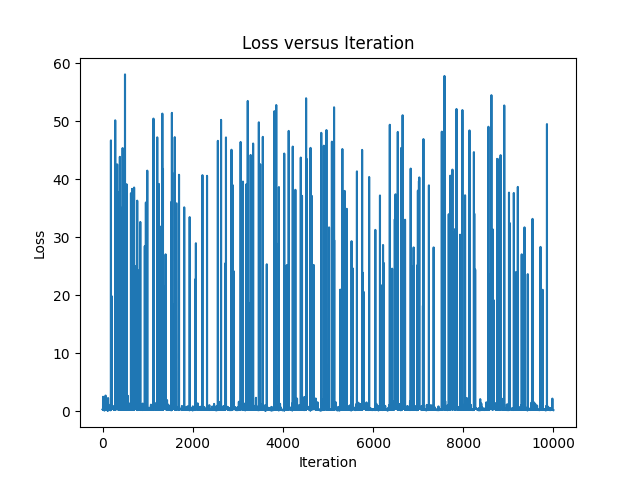
\includegraphics[scale=0.75]{Pure_CNN.png}
        \caption{Loss against iteration for CNN model, trained against a random agent}
        \label{fig:}
    \end{center}
\end{figure}

The CNN value function was trained against a random agent for 10,000 iterations, with 1 iteration being a complete Santorini game. The algorithm used to generate the reward for each state, as well as to backpropagate the loss, is as explained in Section \_\_. The loss displayed in the graph is the cumulative loss for each iteration. From the graph, there is a general decreasing trend, plateauing at a value close to 0.  \par

There are also many “spikes” that can be seen protruding from the general trendline. The model, in these iterations, has not explored these states before, and this results in a state-value that is extremely different from the true state-value, thus contributing to the high loss value for each evaluated state per iteration. The cumulative sum of these losses for that iteration resulted in the spike for 1 iteration. \par

\subsection{Loss against iteration for MCTS Models}
\begin{figure}[H]
    \begin{center}
        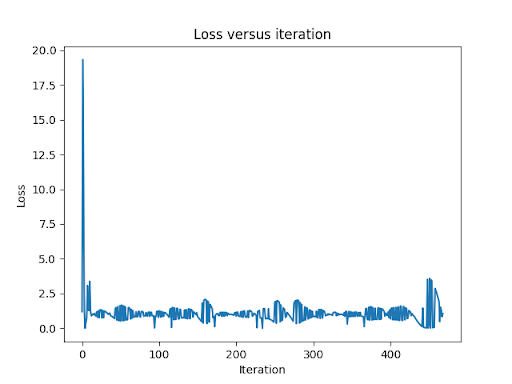
\includegraphics[scale=0.8]{MCTS_ANN.png}
        \caption{Loss against iteration for MCTS ANN model, trained against a random agent}
        \label{fig:}
    \end{center}
\end{figure}

The ANN model was trained using training data produced from a MCTS search tree. In total approximately 500 nodes were explored and with each node there were about 30 simulations. The loss from each node is the mean squared Error loss and is represented in the figure 4. As expected the initial loss is high in the 20s, this is due to the random weights which are intialize whenever a new Neural Network is created. Soon after the loss quickly reduced to lower values. \par

As mentioned earlier, the erratic peaks and falls at later halfs of the training is primarmly due to the fact that new states are encountered and the neural network needs to adjust its weights to account for this novel state.  \par

\begin{figure}[H]
    \begin{center}
        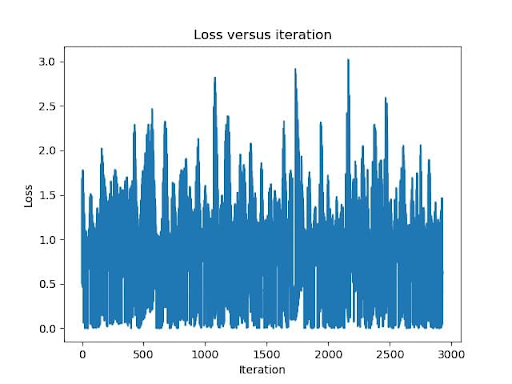
\includegraphics[scale=0.65]{MCTS_CNN.png}
        \caption{Loss against iteration for MCTS CNN model, trained against a random agent}
        \label{fig:}
    \end{center}
\end{figure}
\vspace{-1cm}
The CNN model was trained using training data produced from a MCTS search tree. In total approximately 2800 nodes were explored and with each node there were about 30 simulations. The loss from each node is the mean squared error loss and is represented in the figure 4. However unlike with the ANN, the training loss for the MCTS CNN model is quite different. This can partly be attributed to the fact the the CNN may be overestimate the value of certain features which were encountered in a previous training iterations, and the time for which the MCTS algorithm ran was not long enough for the values of the different states to converge. \par


\begin{table}[H]
    \resizebox{\textwidth}{!}{%
    \begin{tabular}{|c|cccccccccc}
    \hline
    \multicolumn{11}{|c|}{Win Rates}                                                                                                                                                                                                                                                                                                                                                                                                                                                                                                   \\ \hline
                   & \multicolumn{1}{c|}{Random}                     & \multicolumn{1}{c|}{ANN}                        & \multicolumn{1}{c|}{CNN}                        & \multicolumn{1}{c|}{MCTS\_ANN}                  & \multicolumn{1}{c|}{MCTS\_CNN}                  & \multicolumn{1}{c|}{Combined}                   & \multicolumn{1}{c|}{Linear TreeStrap}             & \multicolumn{1}{c|}{Linear RootStrap}             & \multicolumn{1}{c|}{Linear Manual}             & \multicolumn{1}{c|}{Human}                      \\ \hline
    Random         & \cellcolor[HTML]{000000}{\color[HTML]{000000} } & \cellcolor[HTML]{000000}{\color[HTML]{333333} } & \cellcolor[HTML]{000000}{\color[HTML]{333333} } & \cellcolor[HTML]{000000}{\color[HTML]{333333} } & \cellcolor[HTML]{000000}                        & \cellcolor[HTML]{000000}                        & \cellcolor[HTML]{000000}                        & \cellcolor[HTML]{000000}                        & \cellcolor[HTML]{000000}                        & \cellcolor[HTML]{000000}                        \\ \cline{1-2}
    ANN            & \multicolumn{1}{c|}{}                           & \cellcolor[HTML]{000000}                        & \cellcolor[HTML]{000000}{\color[HTML]{333333} } & \cellcolor[HTML]{000000}{\color[HTML]{333333} } & \cellcolor[HTML]{000000}                        & \cellcolor[HTML]{000000}                        & \cellcolor[HTML]{000000}                        & \cellcolor[HTML]{000000}                        & \cellcolor[HTML]{000000}                        & \cellcolor[HTML]{000000}                        \\ \cline{1-3}
    CNN            & \multicolumn{1}{c|}{98\%}                       & \multicolumn{1}{c|}{}                           & \cellcolor[HTML]{000000}{\color[HTML]{000000} } & \cellcolor[HTML]{000000}{\color[HTML]{333333} } & \cellcolor[HTML]{000000}                        & \cellcolor[HTML]{000000}                        & \cellcolor[HTML]{000000}                        & \cellcolor[HTML]{000000}                        & \cellcolor[HTML]{000000}                        & \cellcolor[HTML]{000000}                        \\ \cline{1-4}
    MCTS\_ANN      & \multicolumn{1}{c|}{}                           & \multicolumn{1}{c|}{}                           & \multicolumn{1}{c|}{}                           & \cellcolor[HTML]{000000}{\color[HTML]{000000} } & \cellcolor[HTML]{000000}{\color[HTML]{000000} } & \cellcolor[HTML]{000000}{\color[HTML]{000000} } & \cellcolor[HTML]{000000}{\color[HTML]{000000} } & \cellcolor[HTML]{000000}{\color[HTML]{000000} } & \cellcolor[HTML]{000000}{\color[HTML]{000000} } & \cellcolor[HTML]{000000}{\color[HTML]{000000} } \\ \cline{1-5}
    MCTS\_CNN      & \multicolumn{1}{c|}{}                           & \multicolumn{1}{c|}{}                           & \multicolumn{1}{c|}{}                           & \multicolumn{1}{c|}{}                           & \cellcolor[HTML]{000000}                        & \cellcolor[HTML]{000000}                        & \cellcolor[HTML]{000000}                        & \cellcolor[HTML]{000000}                        & \cellcolor[HTML]{000000}                        & \cellcolor[HTML]{000000}                        \\ \cline{1-6}
    Combined       & \multicolumn{1}{c|}{}                           & \multicolumn{1}{c|}{}                           & \multicolumn{1}{c|}{}                           & \multicolumn{1}{c|}{}                           & \multicolumn{1}{c|}{}                           & \cellcolor[HTML]{000000}{\color[HTML]{000000} } & \cellcolor[HTML]{000000}{\color[HTML]{000000} } & \cellcolor[HTML]{000000}{\color[HTML]{000000} } & \cellcolor[HTML]{000000}{\color[HTML]{000000} } & \cellcolor[HTML]{000000}{\color[HTML]{000000} } \\ \cline{1-7}
    Linear TreeStrap & \multicolumn{1}{c|}{100\%}                    & \multicolumn{1}{c|}{}                           & \multicolumn{1}{c|}{89\%}                       & \multicolumn{1}{c|}{}                           & \multicolumn{1}{c|}{}                           & \multicolumn{1}{c|}{}                           & \cellcolor[HTML]{000000}                        & \cellcolor[HTML]{000000}                        & \cellcolor[HTML]{000000}                        & \cellcolor[HTML]{000000}                        \\ \cline{1-8}
    Linear RootStrap & \multicolumn{1}{c|}{100\%}                    & \multicolumn{1}{c|}{}                           & \multicolumn{1}{c|}{100\%}                      & \multicolumn{1}{c|}{}                           & \multicolumn{1}{c|}{}                           & \multicolumn{1}{c|}{}                           & \multicolumn{1}{c|}{}                           & \cellcolor[HTML]{000000}                        & \cellcolor[HTML]{000000}                        & \cellcolor[HTML]{000000}                        \\ \cline{1-9}
    Linear Manual & \multicolumn{1}{c|}{100\%}                       & \multicolumn{1}{c|}{}                           & \multicolumn{1}{c|}{84\%}                       & \multicolumn{1}{c|}{}                           & \multicolumn{1}{c|}{}                           & \multicolumn{1}{c|}{}                           & \multicolumn{1}{c|}{}                           & \multicolumn{1}{c|}{}                           & \cellcolor[HTML]{000000}                        & \cellcolor[HTML]{000000}                        \\ \cline{1-10}
    Human          & \multicolumn{1}{c|}{100\%}                      & \multicolumn{1}{c|}{}                           & \multicolumn{1}{c|}{}                           & \multicolumn{1}{c|}{}                           & \multicolumn{1}{c|}{}                           & \multicolumn{1}{c|}{}                           & \multicolumn{1}{c|}{}                           & \multicolumn{1}{c|}{}                           & \multicolumn{1}{c|}{}                           & \cellcolor[HTML]{000000}                        \\ \cline{1-10}
    \end{tabular}%
    }
    \caption{Win Rate of Each Agent}
    \label{table:}
\end{table}


\subsection{Limitations of above methods}

\textbf{General Limitaion}
\newline
This study had a few limitations that were common across all methods employed. These limitations restricted further optimization and hyperparameter tuning of the models. This section will be using AlphaGo as a benchmark for model training and optimization, as AlphaGo is seen as one of the most successful agents trained using reinforcement learning for playing a board game. \par

\begin{enumerate}
    \item \textbf{Processing Power}
    \newline
    The CPUs that were used to train the models were extremely limited in processing power. The models were trained mainly on a single CPU. Parallel programming was not employed due to time constraints. The GPUs that were used to perform calculations for the neural networks was a consumer-grade Nvidia GeForce GTX1060. \par

    In comparison, the AlphaGo AI was trained using up to 1920 CPUs. The AlphaGo neural network calculations were also performed on Google’s own proprietary hardware, the Tensor Processing Unit (TPUs), designed specifically for neural network training, which significantly boosted training speed \cite{Mastering the game of Go with deep neural networks and tree search}. \par

    \begin{itemize}
        \item \textbf{Effects on Model Performance}
        \newline
        Limited processing power restricted the hyperparameter tuning that could be done for the various models. \\

        For the CNN model, a kernel size of 3 was used, however, a kernel size of 2 could also be considered. The usage of padding could also have been evaluated. The number of features for feature map generation could not be too large, thus limiting the model’s capability of detecting an increased number of features on the board. All of the above restricted the optimization of the CNN model, as the various permutations of the hyperparameters could not be done to obtain the most optimized and best-performing model. \\

        For the MCTS algorithm it severely increased the run time for one iteration, with our computer specification it would take 7 days of continuous training to be able to construct a moderately adequate search tree for training. This resulted in us having to cut down on some of the core steps of algorithm making a toned version which is only able to search a depth of 8-10. These limitations also led to a reduction in the efficacy of our AI. \\

        For the models relying on minimax search, lack of computing power limited the search depth the models could be trained at to 3, which limits eventual performance. Furthermore, hyperparameter tuning on parameters such as learning rates would be difficult to perform given the long time taken just to train one model.

    \end{itemize}

    \item \textbf{Lack of Professional Games}
    \newline
    Professional games between experts are essential for an agent’s learning, especially in certain methods tried out that are less effective being trained by self-play. Initially, AlphaGo was trained to simulate professional players, and this was done by training it on 30 million moves \cite{Mastering the game of Go with deep neural networks and tree search}. This sped up the learning process, as the agent can learn to play at a decently high level by “mimicking” professionals.   \par

    As Santorini is not played competitively, and does not have a professional competitive scene, there was a lack of data of professional games for the models to be trained on. Thus, the initial training of the models were mostly done using a random agent who made random moves, instead of ones that were logical and “winning” in nature.
    
    \begin{itemize}
        \item \textbf{Effects on Model Performance}
        \newline
        The initial training of agents against a random agent greatly hampered the learning rate of the models. This was due to the randomness in the random agent’s movement, such as not playing a winning move, or moving into a position of less value, which resulted in “false” wins for the agents (as the agents would have lost if it was a “rational”, or human, player), hence giving the agents a positive reward for the states when the states were actually of neutral or negative value. Therefore, this will result in a much slower convergence to the true state-value (for neural networks value function approximator) or the optimal weights for the linear features (for a linear approximator).

        Additionally, the lack of available literature on Santorini also limits the amount of features that can be implemented with regards to the linear value function approximator, given that the ability to come up with informative features is heavily reliant on possessing a deep understanding of the tactics involved in playing Santorini.
    
    \end{itemize}

    \item \textbf{Limitations of CNN model training}
    \newline
    As the CNN was only a value function approximator and does not have a policy network, this severely limited the performance of the CNN against more robust models, such as the linear approximator, which had features such as centrality and number of workers on a certain level, as well as a minimax policy with a certain lookahead depth. There was no lookahead for the CNN as it only evaluated the next possible states (acting like a depth 1 agent), thus not learning to consider opponent moves, as well as learning to prevent the opposition from winning (such as placing a level 4 block to prevent the opponent from winning).  \par

    Training a CNN on only a random agent also prevented it from learning the true state-value, as mentioned in Section \_\_. Attempts to train the CNN against itself also did not succeed, as the loss per iteration did not converge, and its performance was comparable to the CNN model train on the random agent. \par

    Nevertheless, the CNN model did perform well against the random agent, implying that it is learning to win by building “staircases” (moving the worker upwards, and placing consecutive building blocks to build a staircase-like structure).  \par

\end{enumerate}

\section{Conclusion}

\begin{thebibliography}{9}
    \bibitem{Reinforcement learning: An introduction} 
    Sutton, R.S., \& Barto, A.G. 
    \textit{Reinforcement learning: An introduction}. 
    Cambridge (Mass.): The MIT Press.
    
    \bibitem{Why Deep Neural Networks for Function Approximation} 
    Liang, Shiyu, and R. Srikant. 
    \textit{Why Deep Neural Networks for Function Approximation?}. 
    ArXiv:1610.04161 [Cs], Mar. 2017. arXiv.org, http://arxiv.org/abs/1610.04161.

    \bibitem{Mastering the game of Go with deep neural networks and tree search}
    Silver, D., Huang, A., Maddison, C. et al
    \textit{Mastering the game of Go with deep neural networks and tree search}
    Nature 529, 484–489 (2016). https://doi.org/10.1038/nature16961

    \bibitem{Bootstrapping from Game Tree Search}
    Veness, J., Silver, D., Uther, W. T., \& Blair, A.
    \textit{Bootstrapping from Game Tree Search}
    In NIPS (Vol. 19, pp. 1937-1945) (2009, December).

\end{thebibliography}

\end{document}


